%%% figures_standalone.tex
%%% Figures individuelles pour l'article
%%% Compilation: pdflatex figures_standalone.tex

\documentclass[border=5pt]{standalone}
\usepackage{tikz}
\usepackage{pgfplots}
\usepackage{amsmath}
\usepackage{amssymb}

\pgfplotsset{compat=1.18}
\usetikzlibrary{patterns, arrows.meta, decorations.pathreplacing, calc}

% Couleurs
\definecolor{color_std}{RGB}{231, 76, 60}
\definecolor{color_opt}{RGB}{46, 204, 113}
\definecolor{color_bg}{RGB}{236, 240, 241}
\definecolor{color_highlight}{RGB}{241, 196, 15}

\begin{document}

%% ============================================================
%% FIGURE 1: SURVIVAL CURVES
%% ============================================================
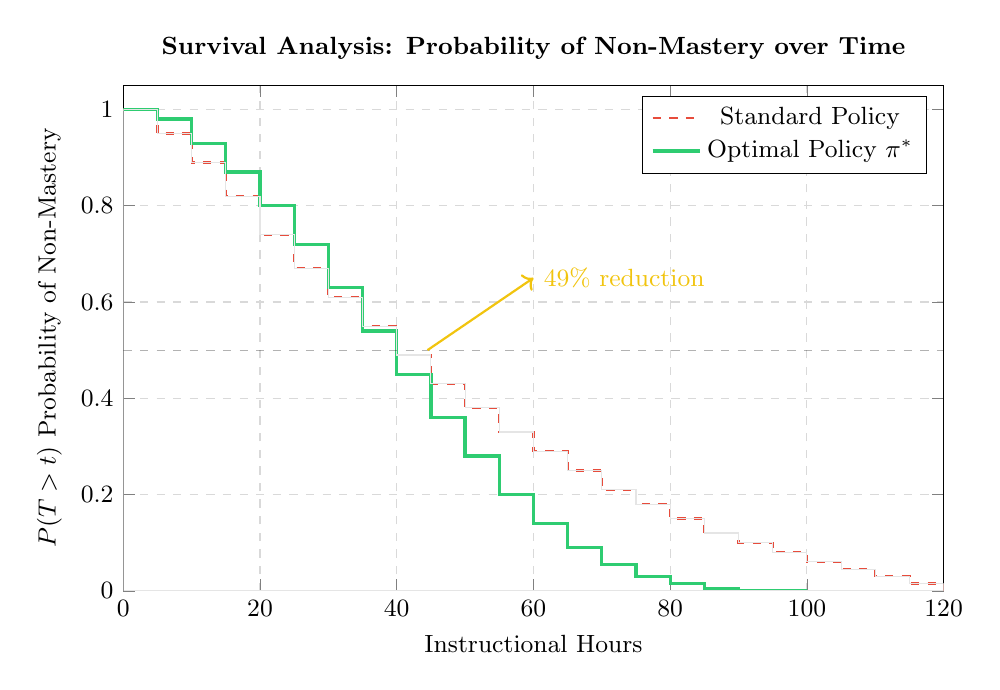
\begin{tikzpicture}
\begin{axis}[
    width=12cm,
    height=8cm,
    xlabel={Instructional Hours},
    ylabel={$P(T > t)$  Probability of Non-Mastery},
    title={Survival Analysis: Probability of Non-Mastery over Time},
    grid=major,
    grid style={dashed, gray!30},
    legend style={at={(0.98,0.98)}, anchor=north east, font=\small},
    xmin=0, xmax=120,
    ymin=0, ymax=1.05,
    tick label style={font=\small},
    label style={font=\small},
    title style={font=\small\bfseries},
]

% Standard policy
\addplot+[
    color=color_std,
    mark=none,
    thick,
    dashed,
    const plot,
]
coordinates {
    (0,1.000)(5,0.950)(10,0.890)(15,0.820)(20,0.740)(25,0.670)
    (30,0.610)(35,0.550)(40,0.490)(45,0.430)(50,0.380)(55,0.330)
    (60,0.290)(65,0.250)(70,0.210)(75,0.180)(80,0.150)(85,0.120)
    (90,0.100)(95,0.080)(100,0.060)(105,0.045)(110,0.030)(115,0.015)(120,0.000)
};

% Optimal policy
\addplot+[
    color=color_opt,
    mark=none,
    very thick,
    const plot,
]
coordinates {
    (0,1.000)(5,0.980)(10,0.930)(15,0.870)(20,0.800)(25,0.720)
    (30,0.630)(35,0.540)(40,0.450)(45,0.360)(50,0.280)(55,0.200)
    (60,0.140)(65,0.090)(70,0.055)(75,0.030)(80,0.015)(85,0.005)
    (90,0.001)(95,0.000)(100,0.000)
};

% Fill between
\addplot[color=gray!20, const plot] coordinates {
    (0,1.000)(5,0.950)(10,0.890)(15,0.820)(20,0.740)(25,0.670)
    (30,0.610)(35,0.550)(40,0.490)(45,0.430)(50,0.380)(55,0.330)
    (60,0.290)(65,0.250)(70,0.210)(75,0.180)(80,0.150)(85,0.120)
    (90,0.100)(95,0.080)(100,0.060)(105,0.045)(110,0.030)(115,0.015)(120,0.000)
} \closedcycle;

% Horizontal line at 0.5
\addplot[black, dashed, opacity=0.3] coordinates {(0,0.5) (120,0.5)};

% Annotation
\draw[color=color_highlight, thick, ->] 
    (axis cs:44.5, 0.5) -- (axis cs:60, 0.65)
    node[right, font=\small, color=color_highlight] {49\% reduction};

\legend{Standard Policy, Optimal Policy $\pi^*$}

\end{axis}
\end{tikzpicture}


%% ============================================================
%% FIGURE 2: CONVERGENCE VELOCITY
%% ============================================================
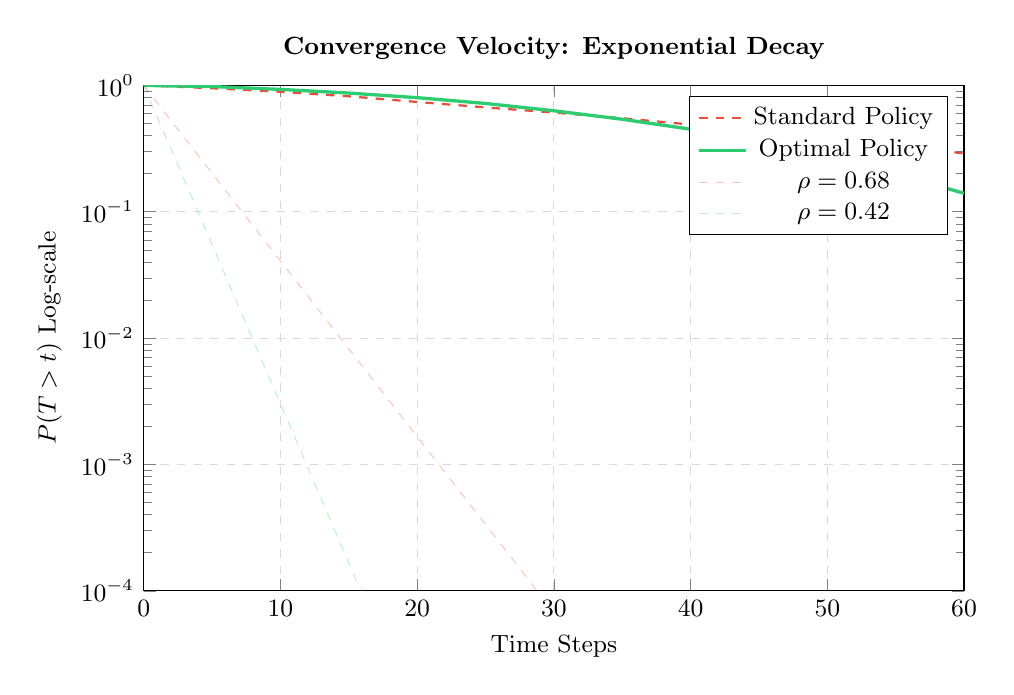
\begin{tikzpicture}
\begin{axis}[
    width=12cm,
    height=8cm,
    xlabel={Time Steps},
    ylabel={$P(T > t)$  Log-scale},
    title={Convergence Velocity: Exponential Decay},
    grid=major,
    grid style={dashed, gray!30},
    legend style={at={(0.98,0.98)}, anchor=north east, font=\small},
    xmin=0, xmax=60,
    ymin=1e-4, ymax=1,
    ymode=log,
    tick label style={font=\small},
    label style={font=\small},
    title style={font=\small\bfseries},
]

% Standard policy
\addplot+[
    color=color_std,
    mark=none,
    dashed,
    thick,
]
coordinates {
    (0,1.000)(5,0.950)(10,0.890)(15,0.820)(20,0.740)(25,0.670)
    (30,0.610)(35,0.550)(40,0.490)(45,0.430)(50,0.380)(55,0.330)(60,0.290)
};

% Optimal policy
\addplot+[
    color=color_opt,
    mark=none,
    very thick,
]
coordinates {
    (0,1.000)(5,0.980)(10,0.930)(15,0.870)(20,0.800)(25,0.720)
    (30,0.630)(35,0.540)(40,0.450)(45,0.360)(50,0.280)(55,0.200)(60,0.140)
};

% Theoretical lines
\addplot[color=color_std, opacity=0.3, domain=0:60, samples=100, dashed]
{exp(-0.32*x)};
\addplot[color=color_opt, opacity=0.3, domain=0:60, samples=100, dashed]
{exp(-0.58*x)};

\legend{Standard Policy, Optimal Policy, $\rho=0.68$, $\rho=0.42$}

\end{axis}
\end{tikzpicture}


%% ============================================================
%% FIGURE 3: EXPECTED TIMES (SIMPLIFIED)
%% ============================================================
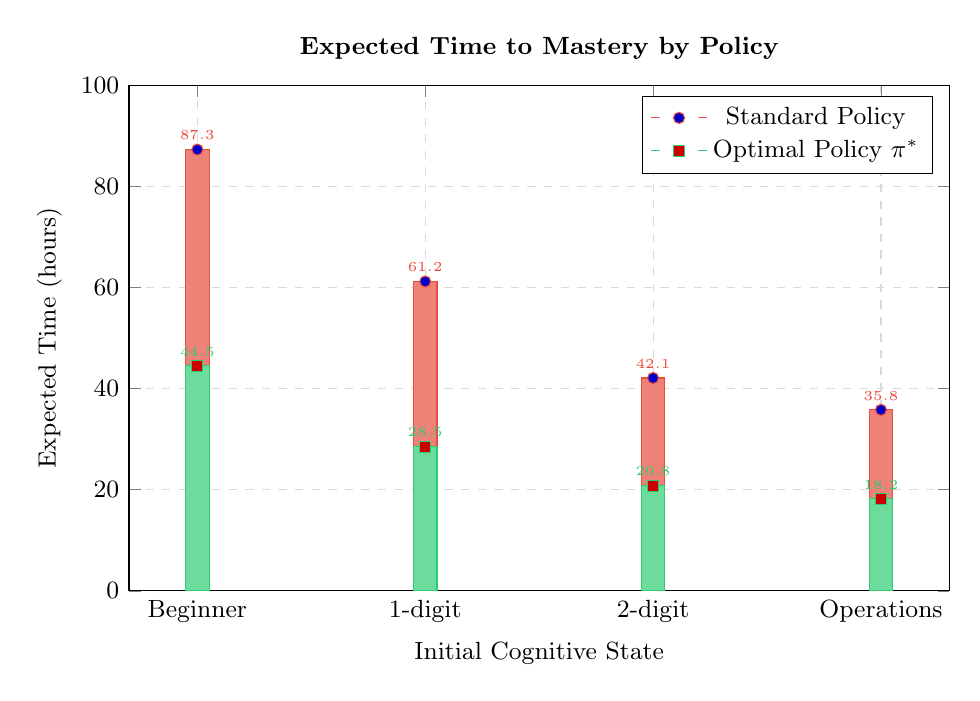
\begin{tikzpicture}
\begin{axis}[
    width=12cm,
    height=8cm,
    xlabel={Initial Cognitive State},
    ylabel={Expected Time (hours)},
    title={Expected Time to Mastery by Policy},
    symbolic x coords={Beginner, 1-digit, 2-digit, Operations},
    xtick=data,
    ymin=0, ymax=100,
    grid=major,
    grid style={dashed, gray!30},
    legend style={at={(0.98,0.98)}, anchor=north east, font=\small},
    tick label style={font=\small},
    label style={font=\small},
    title style={font=\small\bfseries},
]

\addplot+[
    color=color_std,
    ybar,
    bar width=0.3cm,
    fill=color_std!70,
    nodes near coords,
    nodes near coords style={font=\tiny, color=color_std},
]
coordinates {
    (Beginner,87.3)
    (1-digit,61.2)
    (2-digit,42.1)
    (Operations,35.8)
};

\addplot+[
    color=color_opt,
    ybar,
    bar width=0.3cm,
    fill=color_opt!70,
    nodes near coords,
    nodes near coords style={font=\tiny, color=color_opt},
]
coordinates {
    (Beginner,44.5)
    (1-digit,28.5)
    (2-digit,20.8)
    (Operations,18.2)
};

\legend{Standard Policy, Optimal Policy $\pi^*$}

\end{axis}
\end{tikzpicture}


\end{document}